\documentclass[1p]{elsarticle_modified}
%\bibliographystyle{elsarticle-num}

%\usepackage[colorlinks]{hyperref}
%\usepackage{abbrmath_seonhwa} %\Abb, \Ascr, \Acal ,\Abf, \Afrak
\usepackage{amsfonts}
\usepackage{amssymb}
\usepackage{amsmath}
\usepackage{amsthm}
\usepackage{scalefnt}
\usepackage{amsbsy}
\usepackage{kotex}
\usepackage{caption}
\usepackage{subfig}
\usepackage{color}
\usepackage{graphicx}
\usepackage{xcolor} %% white, black, red, green, blue, cyan, magenta, yellow
\usepackage{float}
\usepackage{setspace}
\usepackage{hyperref}

\usepackage{tikz}
\usetikzlibrary{arrows}

\usepackage{multirow}
\usepackage{array} % fixed length table
\usepackage{hhline}

%%%%%%%%%%%%%%%%%%%%%
\makeatletter
\renewcommand*\env@matrix[1][\arraystretch]{%
	\edef\arraystretch{#1}%
	\hskip -\arraycolsep
	\let\@ifnextchar\new@ifnextchar
	\array{*\c@MaxMatrixCols c}}
\makeatother %https://tex.stackexchange.com/questions/14071/how-can-i-increase-the-line-spacing-in-a-matrix
%%%%%%%%%%%%%%%

\usepackage[normalem]{ulem}

\newcommand{\msout}[1]{\ifmmode\text{\sout{\ensuremath{#1}}}\else\sout{#1}\fi}
%SOURCE: \msout is \stkout macro in https://tex.stackexchange.com/questions/20609/strikeout-in-math-mode

\newcommand{\cancel}[1]{
	\ifmmode
	{\color{red}\msout{#1}}
	\else
	{\color{red}\sout{#1}}
	\fi
}

\newcommand{\add}[1]{
	{\color{blue}\uwave{#1}}
}

\newcommand{\replace}[2]{
	\ifmmode
	{\color{red}\msout{#1}}{\color{blue}\uwave{#2}}
	\else
	{\color{red}\sout{#1}}{\color{blue}\uwave{#2}}
	\fi
}

\newcommand{\Sol}{\mathcal{S}} %segment
\newcommand{\D}{D} %diagram
\newcommand{\A}{\mathcal{A}} %arc


%%%%%%%%%%%%%%%%%%%%%%%%%%%%%5 test

\def\sl{\operatorname{\textup{SL}}(2,\Cbb)}
\def\psl{\operatorname{\textup{PSL}}(2,\Cbb)}
\def\quan{\mkern 1mu \triangleright \mkern 1mu}

\theoremstyle{definition}
\newtheorem{thm}{Theorem}[section]
\newtheorem{prop}[thm]{Proposition}
\newtheorem{lem}[thm]{Lemma}
\newtheorem{ques}[thm]{Question}
\newtheorem{cor}[thm]{Corollary}
\newtheorem{defn}[thm]{Definition}
\newtheorem{exam}[thm]{Example}
\newtheorem{rmk}[thm]{Remark}
\newtheorem{alg}[thm]{Algorithm}

\newcommand{\I}{\sqrt{-1}}
\begin{document}

%\begin{frontmatter}
%
%\title{Boundary parabolic representations of knots up to 8 crossings}
%
%%% Group authors per affiliation:
%\author{Yunhi Cho} 
%\address{Department of Mathematics, University of Seoul, Seoul, Korea}
%\ead{yhcho@uos.ac.kr}
%
%
%\author{Seonhwa Kim} %\fnref{s_kim}}
%\address{Center for Geometry and Physics, Institute for Basic Science, Pohang, 37673, Korea}
%\ead{ryeona17@ibs.re.kr}
%
%\author{Hyuk Kim}
%\address{Department of Mathematical Sciences, Seoul National University, Seoul 08826, Korea}
%\ead{hyukkim@snu.ac.kr}
%
%\author{Seokbeom Yoon}
%\address{Department of Mathematical Sciences, Seoul National University, Seoul, 08826,  Korea}
%\ead{sbyoon15@snu.ac.kr}
%
%\begin{abstract}
%We find all boundary parabolic representation of knots up to 8 crossings.
%
%\end{abstract}
%\begin{keyword}
%    \MSC[2010] 57M25 
%\end{keyword}
%
%\end{frontmatter}

%\linenumbers
%\tableofcontents
%
\newcommand\colored[1]{\textcolor{white}{\rule[-0.35ex]{0.8em}{1.4ex}}\kern-0.8em\color{red} #1}%
%\newcommand\colored[1]{\textcolor{white}{ #1}\kern-2.17ex	\textcolor{white}{ #1}\kern-1.81ex	\textcolor{white}{ #1}\kern-2.15ex\color{red}#1	}

{\Large $\underline{12a_{0190}~(K12a_{0190})}$}

\setlength{\tabcolsep}{10pt}
\renewcommand{\arraystretch}{1.6}
\vspace{1cm}\begin{tabular}{m{100pt}>{\centering\arraybackslash}m{274pt}}
\multirow{5}{120pt}{
	\centering
	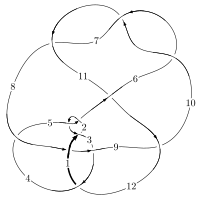
\includegraphics[width=112pt]{../../../GIT/diagram.site/Diagrams/png/991_12a_0190.png}\\
\ \ \ A knot diagram\footnotemark}&
\allowdisplaybreaks
\textbf{Linearized knot diagam} \\
\cline{2-2}
 &
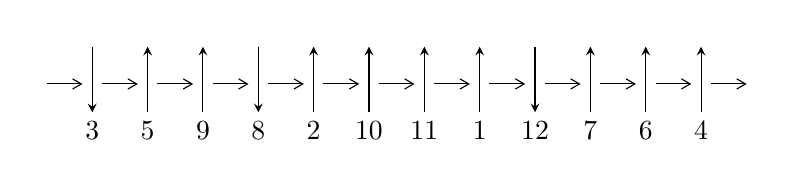
\begin{tikzpicture}[x=20pt, y=17pt]
	% nodes
	\node (C0) at (0, 0) {};
	\node (C1) at (1, 0) {};
	\node (C1U) at (1, +1) {};
	\node (C1D) at (1, -1) {3};

	\node (C2) at (2, 0) {};
	\node (C2U) at (2, +1) {};
	\node (C2D) at (2, -1) {5};

	\node (C3) at (3, 0) {};
	\node (C3U) at (3, +1) {};
	\node (C3D) at (3, -1) {9};

	\node (C4) at (4, 0) {};
	\node (C4U) at (4, +1) {};
	\node (C4D) at (4, -1) {8};

	\node (C5) at (5, 0) {};
	\node (C5U) at (5, +1) {};
	\node (C5D) at (5, -1) {2};

	\node (C6) at (6, 0) {};
	\node (C6U) at (6, +1) {};
	\node (C6D) at (6, -1) {10};

	\node (C7) at (7, 0) {};
	\node (C7U) at (7, +1) {};
	\node (C7D) at (7, -1) {11};

	\node (C8) at (8, 0) {};
	\node (C8U) at (8, +1) {};
	\node (C8D) at (8, -1) {1};

	\node (C9) at (9, 0) {};
	\node (C9U) at (9, +1) {};
	\node (C9D) at (9, -1) {12};

	\node (C10) at (10, 0) {};
	\node (C10U) at (10, +1) {};
	\node (C10D) at (10, -1) {7};

	\node (C11) at (11, 0) {};
	\node (C11U) at (11, +1) {};
	\node (C11D) at (11, -1) {6};

	\node (C12) at (12, 0) {};
	\node (C12U) at (12, +1) {};
	\node (C12D) at (12, -1) {4};
	\node (C13) at (13, 0) {};

	% arrows
	\draw[->,>={angle 60}]
	(C0) edge (C1) (C1) edge (C2) (C2) edge (C3) (C3) edge (C4) (C4) edge (C5) (C5) edge (C6) (C6) edge (C7) (C7) edge (C8) (C8) edge (C9) (C9) edge (C10) (C10) edge (C11) (C11) edge (C12) (C12) edge (C13) ;	\draw[->,>=stealth]
	(C1U) edge (C1D) (C2D) edge (C2U) (C3D) edge (C3U) (C4U) edge (C4D) (C5D) edge (C5U) (C6D) edge (C6U) (C7D) edge (C7U) (C8D) edge (C8U) (C9U) edge (C9D) (C10D) edge (C10U) (C11D) edge (C11U) (C12D) edge (C12U) ;
	\end{tikzpicture} \\
\hhline{~~} \\& 
\textbf{Solving Sequence} \\ \cline{2-2} 
 &
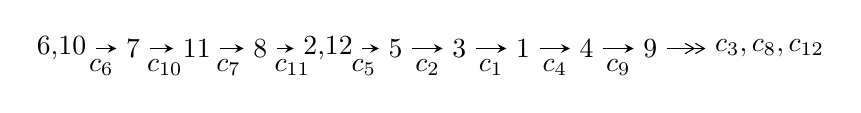
\begin{tikzpicture}[x=23pt, y=7pt]
	% node
	\node (A0) at (-1/8, 0) {6,10};
	\node (A1) at (1, 0) {7};
	\node (A2) at (2, 0) {11};
	\node (A3) at (3, 0) {8};
	\node (A4) at (65/16, 0) {2,12};
	\node (A5) at (41/8, 0) {5};
	\node (A6) at (49/8, 0) {3};
	\node (A7) at (57/8, 0) {1};
	\node (A8) at (65/8, 0) {4};
	\node (A9) at (73/8, 0) {9};
	\node (C1) at (1/2, -1) {$c_{6}$};
	\node (C2) at (3/2, -1) {$c_{10}$};
	\node (C3) at (5/2, -1) {$c_{7}$};
	\node (C4) at (7/2, -1) {$c_{11}$};
	\node (C5) at (37/8, -1) {$c_{5}$};
	\node (C6) at (45/8, -1) {$c_{2}$};
	\node (C7) at (53/8, -1) {$c_{1}$};
	\node (C8) at (61/8, -1) {$c_{4}$};
	\node (C9) at (69/8, -1) {$c_{9}$};
	\node (A10) at (11, 0) {$c_{3},c_{8},c_{12}$};

	% edge
	\draw[->,>=stealth]	
	(A0) edge (A1) (A1) edge (A2) (A2) edge (A3) (A3) edge (A4) (A4) edge (A5) (A5) edge (A6) (A6) edge (A7) (A7) edge (A8) (A8) edge (A9) ;
	\draw[->>,>={angle 60}]	
	(A9) edge (A10);
\end{tikzpicture} \\ 

\end{tabular} \\

\footnotetext{
The image of knot diagram is generated by the software ``\textbf{Draw programme}" developed by Andrew Bartholomew(\url{http://www.layer8.co.uk/maths/draw/index.htm\#Running-draw}), where we modified some parts for our purpose(\url{https://github.com/CATsTAILs/LinksPainter}).
}\phantom \\ \newline 
\centering \textbf{Ideals for irreducible components\footnotemark of $X_{\text{par}}$} 
 
\begin{align*}
I^u_{1}&=\langle 
2.67377\times10^{71} u^{109}-5.17463\times10^{71} u^{108}+\cdots+4.10404\times10^{71} b+5.42742\times10^{71},\\
\phantom{I^u_{1}}&\phantom{= \langle  }-9.81616\times10^{71} u^{109}+1.63462\times10^{72} u^{108}+\cdots+2.05202\times10^{71} a-7.57506\times10^{71},\\
\phantom{I^u_{1}}&\phantom{= \langle  }u^{110}-3 u^{109}+\cdots+8 u-1\rangle \\
I^u_{2}&=\langle 
2 b- a-1,\;a^2+3,\;u+1\rangle \\
\\
\end{align*}
\raggedright * 2 irreducible components of $\dim_{\mathbb{C}}=0$, with total 112 representations.\\
\footnotetext{All coefficients of polynomials are rational numbers. But the coefficients are sometimes approximated in decimal forms when there is not enough margin.}
\newpage
\renewcommand{\arraystretch}{1}
\centering \section*{I. $I^u_{1}= \langle 2.67\times10^{71} u^{109}-5.17\times10^{71} u^{108}+\cdots+4.10\times10^{71} b+5.43\times10^{71},\;-9.82\times10^{71} u^{109}+1.63\times10^{72} u^{108}+\cdots+2.05\times10^{71} a-7.58\times10^{71},\;u^{110}-3 u^{109}+\cdots+8 u-1 \rangle$}
\flushleft \textbf{(i) Arc colorings}\\
\begin{tabular}{m{7pt} m{180pt} m{7pt} m{180pt} }
\flushright $a_{6}=$&$\begin{pmatrix}1\\0\end{pmatrix}$ \\
\flushright $a_{10}=$&$\begin{pmatrix}0\\u\end{pmatrix}$ \\
\flushright $a_{7}=$&$\begin{pmatrix}1\\- u^2\end{pmatrix}$ \\
\flushright $a_{11}=$&$\begin{pmatrix}u\\- u^3+u\end{pmatrix}$ \\
\flushright $a_{8}=$&$\begin{pmatrix}- u^2+1\\u^4-2 u^2\end{pmatrix}$ \\
\flushright $a_{2}=$&$\begin{pmatrix}4.78366 u^{109}-7.96591 u^{108}+\cdots-16.2149 u+3.69151\\-0.651497 u^{109}+1.26086 u^{108}+\cdots+10.2507 u-1.32246\end{pmatrix}$ \\
\flushright $a_{12}=$&$\begin{pmatrix}- u^3+2 u\\- u^3+u\end{pmatrix}$ \\
\flushright $a_{5}=$&$\begin{pmatrix}-14.0684 u^{109}+25.6715 u^{108}+\cdots+96.8437 u-13.6523\\-0.875843 u^{109}+1.66189 u^{108}+\cdots+11.1520 u-2.38600\end{pmatrix}$ \\
\flushright $a_{3}=$&$\begin{pmatrix}-13.3409 u^{109}+24.7528 u^{108}+\cdots+99.6560 u-15.0161\\-1.58470 u^{109}+2.94901 u^{108}+\cdots+15.5277 u-3.08164\end{pmatrix}$ \\
\flushright $a_{1}=$&$\begin{pmatrix}2.29763 u^{109}-3.93043 u^{108}+\cdots-9.56518 u-0.0651181\\0.683728 u^{109}-0.838824 u^{108}+\cdots-0.453193 u-0.136203\end{pmatrix}$ \\
\flushright $a_{4}=$&$\begin{pmatrix}-11.4285 u^{109}+22.4100 u^{108}+\cdots+92.0592 u-13.8943\\3.48936 u^{109}-5.81189 u^{108}+\cdots-16.2207 u+1.70832\end{pmatrix}$ \\
\flushright $a_{9}=$&$\begin{pmatrix}u^7-4 u^5+4 u^3\\u^7-3 u^5+2 u^3+u\end{pmatrix}$\\&\end{tabular}
\flushleft \textbf{(ii) Obstruction class $= -1$}\\~\\
\flushleft \textbf{(iii) Cusp Shapes $= 82.9086 u^{109}-149.372 u^{108}+\cdots-520.277 u+76.7509$}\\~\\
\newpage\renewcommand{\arraystretch}{1}
\flushleft \textbf{(iv) u-Polynomials at the component}\newline \\
\begin{tabular}{m{50pt}|m{274pt}}
Crossings & \hspace{64pt}u-Polynomials at each crossing \\
\hline $$\begin{aligned}c_{1}\end{aligned}$$&$\begin{aligned}
&u^{110}+42 u^{109}+\cdots-41 u+1
\end{aligned}$\\
\hline $$\begin{aligned}c_{2},c_{5}\end{aligned}$$&$\begin{aligned}
&u^{110}+2 u^{109}+\cdots-5 u+1
\end{aligned}$\\
\hline $$\begin{aligned}c_{3}\end{aligned}$$&$\begin{aligned}
&u^{110}+2 u^{109}+\cdots+102407 u-11029
\end{aligned}$\\
\hline $$\begin{aligned}c_{4}\end{aligned}$$&$\begin{aligned}
&u^{110}+4 u^{109}+\cdots-120613 u+16231
\end{aligned}$\\
\hline $$\begin{aligned}c_{6},c_{7},c_{10}\end{aligned}$$&$\begin{aligned}
&u^{110}-3 u^{109}+\cdots+8 u-1
\end{aligned}$\\
\hline $$\begin{aligned}c_{8}\end{aligned}$$&$\begin{aligned}
&u^{110}-7 u^{109}+\cdots+4 u^2-1
\end{aligned}$\\
\hline $$\begin{aligned}c_{9}\end{aligned}$$&$\begin{aligned}
&u^{110}-21 u^{109}+\cdots-3668038 u+132529
\end{aligned}$\\
\hline $$\begin{aligned}c_{11}\end{aligned}$$&$\begin{aligned}
&u^{110}+3 u^{109}+\cdots-60672 u+14144
\end{aligned}$\\
\hline $$\begin{aligned}c_{12}\end{aligned}$$&$\begin{aligned}
&u^{110}+11 u^{109}+\cdots-4 u+4
\end{aligned}$\\
\hline
\end{tabular}\\~\\
\newpage\renewcommand{\arraystretch}{1}
\flushleft \textbf{(v) Riley Polynomials at the component}\newline \\
\begin{tabular}{m{50pt}|m{274pt}}
Crossings & \hspace{64pt}Riley Polynomials at each crossing \\
\hline $$\begin{aligned}c_{1}\end{aligned}$$&$\begin{aligned}
&y^{110}+54 y^{109}+\cdots-249 y+1
\end{aligned}$\\
\hline $$\begin{aligned}c_{2},c_{5}\end{aligned}$$&$\begin{aligned}
&y^{110}+42 y^{109}+\cdots-41 y+1
\end{aligned}$\\
\hline $$\begin{aligned}c_{3}\end{aligned}$$&$\begin{aligned}
&y^{110}-142 y^{109}+\cdots-10478723377 y+121638841
\end{aligned}$\\
\hline $$\begin{aligned}c_{4}\end{aligned}$$&$\begin{aligned}
&y^{110}-90 y^{109}+\cdots-24945269141 y+263445361
\end{aligned}$\\
\hline $$\begin{aligned}c_{6},c_{7},c_{10}\end{aligned}$$&$\begin{aligned}
&y^{110}-101 y^{109}+\cdots-8 y+1
\end{aligned}$\\
\hline $$\begin{aligned}c_{8}\end{aligned}$$&$\begin{aligned}
&y^{110}-13 y^{109}+\cdots-8 y+1
\end{aligned}$\\
\hline $$\begin{aligned}c_{9}\end{aligned}$$&$\begin{aligned}
&y^{110}+63 y^{109}+\cdots+713896960236 y+17563935841
\end{aligned}$\\
\hline $$\begin{aligned}c_{11}\end{aligned}$$&$\begin{aligned}
&y^{110}-23 y^{109}+\cdots-7863217792 y+200052736
\end{aligned}$\\
\hline $$\begin{aligned}c_{12}\end{aligned}$$&$\begin{aligned}
&y^{110}-15 y^{109}+\cdots-264 y+16
\end{aligned}$\\
\hline
\end{tabular}\\~\\
\newpage\flushleft \textbf{(vi) Complex Volumes and Cusp Shapes}
$$\begin{array}{c|c|c}  
\text{Solutions to }I^u_{1}& \I (\text{vol} + \sqrt{-1}CS) & \text{Cusp shape}\\
 \hline 
\begin{aligned}
u &= \phantom{-}1.042430 + 0.304760 I \\
a &= \phantom{-}0.69080 - 1.25394 I \\
b &= -0.490951 - 0.711163 I\end{aligned}
 & \phantom{-}1.73683 + 1.13820 I & \phantom{-0.000000 } 0 \\ \hline\begin{aligned}
u &= \phantom{-}1.042430 - 0.304760 I \\
a &= \phantom{-}0.69080 + 1.25394 I \\
b &= -0.490951 + 0.711163 I\end{aligned}
 & \phantom{-}1.73683 - 1.13820 I & \phantom{-0.000000 } 0 \\ \hline\begin{aligned}
u &= \phantom{-}0.709787 + 0.529952 I \\
a &= \phantom{-}0.094658 + 0.769532 I \\
b &= -0.612347 + 0.859094 I\end{aligned}
 & \phantom{-}3.00793 - 1.60581 I & \phantom{-0.000000 } 0 \\ \hline\begin{aligned}
u &= \phantom{-}0.709787 - 0.529952 I \\
a &= \phantom{-}0.094658 - 0.769532 I \\
b &= -0.612347 - 0.859094 I\end{aligned}
 & \phantom{-}3.00793 + 1.60581 I & \phantom{-0.000000 } 0 \\ \hline\begin{aligned}
u &= \phantom{-}0.633711 + 0.588741 I \\
a &= \phantom{-}0.668832 - 1.023250 I \\
b &= -0.615338 - 0.830644 I\end{aligned}
 & \phantom{-}3.09579 + 3.22900 I & \phantom{-0.000000 } 0 \\ \hline\begin{aligned}
u &= \phantom{-}0.633711 - 0.588741 I \\
a &= \phantom{-}0.668832 + 1.023250 I \\
b &= -0.615338 + 0.830644 I\end{aligned}
 & \phantom{-}3.09579 - 3.22900 I & \phantom{-0.000000 } 0 \\ \hline\begin{aligned}
u &= -1.136620 + 0.182300 I \\
a &= -0.14401 - 1.78120 I \\
b &= -0.070153 - 1.175620 I\end{aligned}
 & -2.43949 - 3.79745 I & \phantom{-0.000000 } 0 \\ \hline\begin{aligned}
u &= -1.136620 - 0.182300 I \\
a &= -0.14401 + 1.78120 I \\
b &= -0.070153 + 1.175620 I\end{aligned}
 & -2.43949 + 3.79745 I & \phantom{-0.000000 } 0 \\ \hline\begin{aligned}
u &= \phantom{-}0.356416 + 0.767376 I \\
a &= \phantom{-}0.95148 - 1.95836 I \\
b &= -0.613775 - 0.920723 I\end{aligned}
 & \phantom{-}1.82712 + 6.13376 I & \phantom{-0.000000 } 0 \\ \hline\begin{aligned}
u &= \phantom{-}0.356416 - 0.767376 I \\
a &= \phantom{-}0.95148 + 1.95836 I \\
b &= -0.613775 + 0.920723 I\end{aligned}
 & \phantom{-}1.82712 - 6.13376 I & \phantom{-0.000000 } 0\\
 \hline 
 \end{array}$$\newpage$$\begin{array}{c|c|c}  
\text{Solutions to }I^u_{1}& \I (\text{vol} + \sqrt{-1}CS) & \text{Cusp shape}\\
 \hline 
\begin{aligned}
u &= \phantom{-}0.406637 + 0.732719 I \\
a &= -0.474129 + 0.329964 I \\
b &= -0.605411 + 0.753946 I\end{aligned}
 & \phantom{-}2.34496 + 1.30819 I & \phantom{-0.000000 } 0 \\ \hline\begin{aligned}
u &= \phantom{-}0.406637 - 0.732719 I \\
a &= -0.474129 - 0.329964 I \\
b &= -0.605411 - 0.753946 I\end{aligned}
 & \phantom{-}2.34496 - 1.30819 I & \phantom{-0.000000 } 0 \\ \hline\begin{aligned}
u &= -0.631106 + 0.523418 I \\
a &= \phantom{-}0.063499 - 0.929955 I \\
b &= -0.693197 - 1.091710 I\end{aligned}
 & \phantom{-}3.03970 + 10.45680 I & \phantom{-0.000000 } 0 \\ \hline\begin{aligned}
u &= -0.631106 - 0.523418 I \\
a &= \phantom{-}0.063499 + 0.929955 I \\
b &= -0.693197 + 1.091710 I\end{aligned}
 & \phantom{-}3.03970 - 10.45680 I & \phantom{-0.000000 } 0 \\ \hline\begin{aligned}
u &= -0.357210 + 0.732588 I \\
a &= \phantom{-}1.23601 + 2.38787 I \\
b &= -0.697975 + 1.114660 I\end{aligned}
 & \phantom{-}2.0566 - 14.7635 I & \phantom{-0.000000 } 0 \\ \hline\begin{aligned}
u &= -0.357210 - 0.732588 I \\
a &= \phantom{-}1.23601 - 2.38787 I \\
b &= -0.697975 - 1.114660 I\end{aligned}
 & \phantom{-}2.0566 + 14.7635 I & \phantom{-0.000000 } 0 \\ \hline\begin{aligned}
u &= -0.365820 + 0.709983 I \\
a &= -0.877302 + 0.431752 I \\
b &= -0.924219 - 0.528395 I\end{aligned}
 & \phantom{-}3.85584 - 8.80943 I & \phantom{-}6.00000 + 6.63181 I \\ \hline\begin{aligned}
u &= -0.365820 - 0.709983 I \\
a &= -0.877302 - 0.431752 I \\
b &= -0.924219 + 0.528395 I\end{aligned}
 & \phantom{-}3.85584 + 8.80943 I & \phantom{-}6.00000 - 6.63181 I \\ \hline\begin{aligned}
u &= \phantom{-}1.196860 + 0.125400 I \\
a &= \phantom{-}0.679124 - 0.504764 I \\
b &= -0.287494 - 0.066047 I\end{aligned}
 & \phantom{-}1.85030 + 0.56407 I & \phantom{-0.000000 } 0 \\ \hline\begin{aligned}
u &= \phantom{-}1.196860 - 0.125400 I \\
a &= \phantom{-}0.679124 + 0.504764 I \\
b &= -0.287494 + 0.066047 I\end{aligned}
 & \phantom{-}1.85030 - 0.56407 I & \phantom{-0.000000 } 0\\
 \hline 
 \end{array}$$\newpage$$\begin{array}{c|c|c}  
\text{Solutions to }I^u_{1}& \I (\text{vol} + \sqrt{-1}CS) & \text{Cusp shape}\\
 \hline 
\begin{aligned}
u &= \phantom{-}1.207530 + 0.036111 I \\
a &= -2.05692 + 4.49642 I \\
b &= \phantom{-}0.475367 + 0.904372 I\end{aligned}
 & \phantom{-}2.18862 + 2.29145 I & \phantom{-0.000000 } 0 \\ \hline\begin{aligned}
u &= \phantom{-}1.207530 - 0.036111 I \\
a &= -2.05692 - 4.49642 I \\
b &= \phantom{-}0.475367 - 0.904372 I\end{aligned}
 & \phantom{-}2.18862 - 2.29145 I & \phantom{-0.000000 } 0 \\ \hline\begin{aligned}
u &= -0.585644 + 0.524890 I \\
a &= \phantom{-}0.307417 + 0.678703 I \\
b &= -0.887496 + 0.553841 I\end{aligned}
 & \phantom{-}4.68466 + 4.61363 I & \phantom{-}10.47045 + 0. I\phantom{ +0.000000I} \\ \hline\begin{aligned}
u &= -0.585644 - 0.524890 I \\
a &= \phantom{-}0.307417 - 0.678703 I \\
b &= -0.887496 - 0.553841 I\end{aligned}
 & \phantom{-}4.68466 - 4.61363 I & \phantom{-}10.47045 + 0. I\phantom{ +0.000000I} \\ \hline\begin{aligned}
u &= \phantom{-}1.167380 + 0.336331 I \\
a &= -0.364740 + 0.861422 I \\
b &= -0.564442 + 0.983855 I\end{aligned}
 & \phantom{-}0.77242 - 3.22559 I & \phantom{-0.000000 } 0 \\ \hline\begin{aligned}
u &= \phantom{-}1.167380 - 0.336331 I \\
a &= -0.364740 - 0.861422 I \\
b &= -0.564442 - 0.983855 I\end{aligned}
 & \phantom{-}0.77242 + 3.22559 I & \phantom{-0.000000 } 0 \\ \hline\begin{aligned}
u &= \phantom{-}0.022669 + 0.764528 I \\
a &= -0.28681 - 2.41502 I \\
b &= -0.590058 - 1.033690 I\end{aligned}
 & -2.73847 + 7.20991 I & \phantom{-}2.16879 - 8.38863 I \\ \hline\begin{aligned}
u &= \phantom{-}0.022669 - 0.764528 I \\
a &= -0.28681 + 2.41502 I \\
b &= -0.590058 + 1.033690 I\end{aligned}
 & -2.73847 - 7.20991 I & \phantom{-}2.16879 + 8.38863 I \\ \hline\begin{aligned}
u &= -1.240340 + 0.100015 I \\
a &= -0.54389 - 1.88615 I \\
b &= \phantom{-}0.554895 - 1.160570 I\end{aligned}
 & \phantom{-}2.33423 - 4.86971 I & \phantom{-0.000000 } 0 \\ \hline\begin{aligned}
u &= -1.240340 - 0.100015 I \\
a &= -0.54389 + 1.88615 I \\
b &= \phantom{-}0.554895 + 1.160570 I\end{aligned}
 & \phantom{-}2.33423 + 4.86971 I & \phantom{-0.000000 } 0\\
 \hline 
 \end{array}$$\newpage$$\begin{array}{c|c|c}  
\text{Solutions to }I^u_{1}& \I (\text{vol} + \sqrt{-1}CS) & \text{Cusp shape}\\
 \hline 
\begin{aligned}
u &= -1.214290 + 0.306199 I \\
a &= \phantom{-}1.03227 + 1.77137 I \\
b &= -0.618109 + 1.069640 I\end{aligned}
 & \phantom{-}1.06963 - 11.08770 I & \phantom{-0.000000 } 0 \\ \hline\begin{aligned}
u &= -1.214290 - 0.306199 I \\
a &= \phantom{-}1.03227 - 1.77137 I \\
b &= -0.618109 - 1.069640 I\end{aligned}
 & \phantom{-}1.06963 + 11.08770 I & \phantom{-0.000000 } 0 \\ \hline\begin{aligned}
u &= -0.310953 + 0.669600 I \\
a &= -1.14221 - 2.41787 I \\
b &= \phantom{-}0.069246 - 1.279980 I\end{aligned}
 & -3.10384 - 6.63654 I & \phantom{-}1.93522 + 9.14652 I \\ \hline\begin{aligned}
u &= -0.310953 - 0.669600 I \\
a &= -1.14221 + 2.41787 I \\
b &= \phantom{-}0.069246 + 1.279980 I\end{aligned}
 & -3.10384 + 6.63654 I & \phantom{-}1.93522 - 9.14652 I \\ \hline\begin{aligned}
u &= -1.244590 + 0.256295 I \\
a &= -0.253010 + 0.080772 I \\
b &= -0.743437 - 0.435345 I\end{aligned}
 & \phantom{-}2.87173 - 5.93046 I & \phantom{-0.000000 } 0 \\ \hline\begin{aligned}
u &= -1.244590 - 0.256295 I \\
a &= -0.253010 - 0.080772 I \\
b &= -0.743437 + 0.435345 I\end{aligned}
 & \phantom{-}2.87173 + 5.93046 I & \phantom{-0.000000 } 0 \\ \hline\begin{aligned}
u &= \phantom{-}1.279450 + 0.018733 I \\
a &= \phantom{-}1.00242 + 1.52201 I \\
b &= \phantom{-}0.389202 - 0.762314 I\end{aligned}
 & \phantom{-}2.64749 - 1.42674 I & \phantom{-0.000000 } 0 \\ \hline\begin{aligned}
u &= \phantom{-}1.279450 - 0.018733 I \\
a &= \phantom{-}1.00242 - 1.52201 I \\
b &= \phantom{-}0.389202 + 0.762314 I\end{aligned}
 & \phantom{-}2.64749 + 1.42674 I & \phantom{-0.000000 } 0 \\ \hline\begin{aligned}
u &= -0.350653 + 0.619552 I \\
a &= -1.34360 - 2.38427 I \\
b &= \phantom{-}0.735903 - 1.161470 I\end{aligned}
 & \phantom{-}1.54460 - 6.34301 I & \phantom{-}9.4689 + 11.6215 I \\ \hline\begin{aligned}
u &= -0.350653 - 0.619552 I \\
a &= -1.34360 + 2.38427 I \\
b &= \phantom{-}0.735903 + 1.161470 I\end{aligned}
 & \phantom{-}1.54460 + 6.34301 I & \phantom{-}9.4689 - 11.6215 I\\
 \hline 
 \end{array}$$\newpage$$\begin{array}{c|c|c}  
\text{Solutions to }I^u_{1}& \I (\text{vol} + \sqrt{-1}CS) & \text{Cusp shape}\\
 \hline 
\begin{aligned}
u &= -1.293700 + 0.044391 I \\
a &= -0.367167 - 0.309954 I \\
b &= \phantom{-}0.835764 - 0.804452 I\end{aligned}
 & \phantom{-}4.82731 - 3.06865 I & \phantom{-0.000000 } 0 \\ \hline\begin{aligned}
u &= -1.293700 - 0.044391 I \\
a &= -0.367167 + 0.309954 I \\
b &= \phantom{-}0.835764 + 0.804452 I\end{aligned}
 & \phantom{-}4.82731 + 3.06865 I & \phantom{-0.000000 } 0 \\ \hline\begin{aligned}
u &= -0.382833 + 0.589995 I \\
a &= -0.159594 - 1.232590 I \\
b &= \phantom{-}1.001380 - 0.537434 I\end{aligned}
 & \phantom{-}3.62807 - 3.58901 I & \phantom{-}15.0481 + 7.4264 I \\ \hline\begin{aligned}
u &= -0.382833 - 0.589995 I \\
a &= -0.159594 + 1.232590 I \\
b &= \phantom{-}1.001380 + 0.537434 I\end{aligned}
 & \phantom{-}3.62807 + 3.58901 I & \phantom{-}15.0481 - 7.4264 I \\ \hline\begin{aligned}
u &= \phantom{-}0.071201 + 0.692830 I \\
a &= -0.573489 + 1.010040 I \\
b &= -0.584487 + 0.449534 I\end{aligned}
 & -1.16620 + 2.47035 I & \phantom{-}4.14055 - 4.42574 I \\ \hline\begin{aligned}
u &= \phantom{-}0.071201 - 0.692830 I \\
a &= -0.573489 - 1.010040 I \\
b &= -0.584487 - 0.449534 I\end{aligned}
 & -1.16620 - 2.47035 I & \phantom{-}4.14055 + 4.42574 I \\ \hline\begin{aligned}
u &= -0.401400 + 0.560284 I \\
a &= \phantom{-}0.737726 - 0.734520 I \\
b &= \phantom{-}0.994561 + 0.430873 I\end{aligned}
 & \phantom{-}3.73746 - 0.06066 I & \phantom{-}15.7625 + 0.6829 I \\ \hline\begin{aligned}
u &= -0.401400 - 0.560284 I \\
a &= \phantom{-}0.737726 + 0.734520 I \\
b &= \phantom{-}0.994561 - 0.430873 I\end{aligned}
 & \phantom{-}3.73746 + 0.06066 I & \phantom{-}15.7625 - 0.6829 I \\ \hline\begin{aligned}
u &= -1.31180\phantom{ +0.000000I} \\
a &= \phantom{-}0.293323\phantom{ +0.000000I} \\
b &= \phantom{-}0.836540\phantom{ +0.000000I}\end{aligned}
 & \phantom{-}5.58489\phantom{ +0.000000I} & \phantom{-0.000000 } 0 \\ \hline\begin{aligned}
u &= \phantom{-}1.293690 + 0.255561 I \\
a &= \phantom{-}1.56944 - 1.41967 I \\
b &= -0.229918 - 1.049980 I\end{aligned}
 & -1.21197 + 2.79771 I & \phantom{-0.000000 } 0\\
 \hline 
 \end{array}$$\newpage$$\begin{array}{c|c|c}  
\text{Solutions to }I^u_{1}& \I (\text{vol} + \sqrt{-1}CS) & \text{Cusp shape}\\
 \hline 
\begin{aligned}
u &= \phantom{-}1.293690 - 0.255561 I \\
a &= \phantom{-}1.56944 + 1.41967 I \\
b &= -0.229918 + 1.049980 I\end{aligned}
 & -1.21197 - 2.79771 I & \phantom{-0.000000 } 0 \\ \hline\begin{aligned}
u &= \phantom{-}0.371452 + 0.569739 I \\
a &= \phantom{-}0.610361 + 0.152921 I \\
b &= \phantom{-}0.213712 + 0.096656 I\end{aligned}
 & \phantom{-}0.87797 + 1.75361 I & \phantom{-}4.00098 - 4.23879 I \\ \hline\begin{aligned}
u &= \phantom{-}0.371452 - 0.569739 I \\
a &= \phantom{-}0.610361 - 0.152921 I \\
b &= \phantom{-}0.213712 - 0.096656 I\end{aligned}
 & \phantom{-}0.87797 - 1.75361 I & \phantom{-}4.00098 + 4.23879 I \\ \hline\begin{aligned}
u &= \phantom{-}0.203337 + 0.648436 I \\
a &= \phantom{-}0.22434 + 1.74473 I \\
b &= -0.070051 + 0.627424 I\end{aligned}
 & -0.91786 + 2.31127 I & \phantom{-}2.88014 - 5.91888 I \\ \hline\begin{aligned}
u &= \phantom{-}0.203337 - 0.648436 I \\
a &= \phantom{-}0.22434 - 1.74473 I \\
b &= -0.070051 - 0.627424 I\end{aligned}
 & -0.91786 - 2.31127 I & \phantom{-}2.88014 + 5.91888 I \\ \hline\begin{aligned}
u &= -0.090046 + 0.672441 I \\
a &= \phantom{-}0.91087 + 2.89991 I \\
b &= -0.146928 + 1.096740 I\end{aligned}
 & -5.51656 + 0.56608 I & -3.17725 - 0.33604 I \\ \hline\begin{aligned}
u &= -0.090046 - 0.672441 I \\
a &= \phantom{-}0.91087 - 2.89991 I \\
b &= -0.146928 - 1.096740 I\end{aligned}
 & -5.51656 - 0.56608 I & -3.17725 + 0.33604 I \\ \hline\begin{aligned}
u &= \phantom{-}0.331204 + 0.577743 I \\
a &= -4.23259 + 1.33722 I \\
b &= \phantom{-}0.545491 + 0.882798 I\end{aligned}
 & \phantom{-}0.54533 + 3.82916 I & -12.0407 + 14.8512 I \\ \hline\begin{aligned}
u &= \phantom{-}0.331204 - 0.577743 I \\
a &= -4.23259 - 1.33722 I \\
b &= \phantom{-}0.545491 - 0.882798 I\end{aligned}
 & \phantom{-}0.54533 - 3.82916 I & -12.0407 - 14.8512 I \\ \hline\begin{aligned}
u &= -0.412605 + 0.499950 I \\
a &= \phantom{-}0.487656 + 0.457214 I \\
b &= \phantom{-}0.760775 + 1.087850 I\end{aligned}
 & \phantom{-}1.96482 + 2.78043 I & \phantom{-}11.54120 - 4.22354 I\\
 \hline 
 \end{array}$$\newpage$$\begin{array}{c|c|c}  
\text{Solutions to }I^u_{1}& \I (\text{vol} + \sqrt{-1}CS) & \text{Cusp shape}\\
 \hline 
\begin{aligned}
u &= -0.412605 - 0.499950 I \\
a &= \phantom{-}0.487656 - 0.457214 I \\
b &= \phantom{-}0.760775 - 1.087850 I\end{aligned}
 & \phantom{-}1.96482 - 2.78043 I & \phantom{-}11.54120 + 4.22354 I \\ \hline\begin{aligned}
u &= \phantom{-}0.349722 + 0.536822 I \\
a &= -1.56624 + 1.89326 I \\
b &= \phantom{-}0.544235 - 0.835676 I\end{aligned}
 & \phantom{-}0.698976 - 0.541114 I & -17.8322 - 3.1413 I \\ \hline\begin{aligned}
u &= \phantom{-}0.349722 - 0.536822 I \\
a &= -1.56624 - 1.89326 I \\
b &= \phantom{-}0.544235 + 0.835676 I\end{aligned}
 & \phantom{-}0.698976 + 0.541114 I & -17.8322 + 3.1413 I \\ \hline\begin{aligned}
u &= -0.524889 + 0.356431 I \\
a &= \phantom{-}0.88263 + 1.38930 I \\
b &= \phantom{-}0.089364 + 1.183890 I\end{aligned}
 & -2.05836 + 3.02608 I & \phantom{-}4.11780 - 3.31029 I \\ \hline\begin{aligned}
u &= -0.524889 - 0.356431 I \\
a &= \phantom{-}0.88263 - 1.38930 I \\
b &= \phantom{-}0.089364 - 1.183890 I\end{aligned}
 & -2.05836 - 3.02608 I & \phantom{-}4.11780 + 3.31029 I \\ \hline\begin{aligned}
u &= -1.394820 + 0.206569 I \\
a &= \phantom{-}1.17315 + 1.83804 I \\
b &= \phantom{-}0.305575 + 0.879647 I\end{aligned}
 & \phantom{-}4.85990 - 2.36800 I & \phantom{-0.000000 } 0 \\ \hline\begin{aligned}
u &= -1.394820 - 0.206569 I \\
a &= \phantom{-}1.17315 - 1.83804 I \\
b &= \phantom{-}0.305575 - 0.879647 I\end{aligned}
 & \phantom{-}4.85990 + 2.36800 I & \phantom{-0.000000 } 0 \\ \hline\begin{aligned}
u &= -1.39245 + 0.25151 I \\
a &= -0.049930 - 1.221160 I \\
b &= \phantom{-}0.005383 - 0.793309 I\end{aligned}
 & \phantom{-}4.20117 - 5.58561 I & \phantom{-0.000000 } 0 \\ \hline\begin{aligned}
u &= -1.39245 - 0.25151 I \\
a &= -0.049930 + 1.221160 I \\
b &= \phantom{-}0.005383 + 0.793309 I\end{aligned}
 & \phantom{-}4.20117 + 5.58561 I & \phantom{-0.000000 } 0 \\ \hline\begin{aligned}
u &= \phantom{-}0.223965 + 0.535065 I \\
a &= \phantom{-}2.24434 - 3.62037 I \\
b &= \phantom{-}0.388240 - 0.839913 I\end{aligned}
 & -0.341249 - 0.362728 I & \phantom{-}9.62962 + 1.11519 I\\
 \hline 
 \end{array}$$\newpage$$\begin{array}{c|c|c}  
\text{Solutions to }I^u_{1}& \I (\text{vol} + \sqrt{-1}CS) & \text{Cusp shape}\\
 \hline 
\begin{aligned}
u &= \phantom{-}0.223965 - 0.535065 I \\
a &= \phantom{-}2.24434 + 3.62037 I \\
b &= \phantom{-}0.388240 + 0.839913 I\end{aligned}
 & -0.341249 + 0.362728 I & \phantom{-}9.62962 - 1.11519 I \\ \hline\begin{aligned}
u &= \phantom{-}1.41580 + 0.16623 I \\
a &= \phantom{-}0.693712 - 0.468034 I \\
b &= \phantom{-}0.232628 - 1.242180 I\end{aligned}
 & \phantom{-}3.80684 - 1.07968 I & \phantom{-0.000000 } 0 \\ \hline\begin{aligned}
u &= \phantom{-}1.41580 - 0.16623 I \\
a &= \phantom{-}0.693712 + 0.468034 I \\
b &= \phantom{-}0.232628 + 1.242180 I\end{aligned}
 & \phantom{-}3.80684 + 1.07968 I & \phantom{-0.000000 } 0 \\ \hline\begin{aligned}
u &= -1.42866 + 0.21209 I \\
a &= -1.63529 - 1.87231 I \\
b &= \phantom{-}0.577657 + 0.826939 I\end{aligned}
 & \phantom{-}6.39608 - 2.25864 I & \phantom{-0.000000 } 0 \\ \hline\begin{aligned}
u &= -1.42866 - 0.21209 I \\
a &= -1.63529 + 1.87231 I \\
b &= \phantom{-}0.577657 - 0.826939 I\end{aligned}
 & \phantom{-}6.39608 + 2.25864 I & \phantom{-0.000000 } 0 \\ \hline\begin{aligned}
u &= -1.42691 + 0.22647 I \\
a &= -3.76630 - 0.47368 I \\
b &= \phantom{-}0.569164 - 0.893401 I\end{aligned}
 & \phantom{-}6.18316 - 6.81181 I & \phantom{-0.000000 } 0 \\ \hline\begin{aligned}
u &= -1.42691 - 0.22647 I \\
a &= -3.76630 + 0.47368 I \\
b &= \phantom{-}0.569164 + 0.893401 I\end{aligned}
 & \phantom{-}6.18316 + 6.81181 I & \phantom{-0.000000 } 0 \\ \hline\begin{aligned}
u &= \phantom{-}1.42542 + 0.25767 I \\
a &= -1.26859 + 1.03129 I \\
b &= \phantom{-}0.084417 + 1.321020 I\end{aligned}
 & \phantom{-}2.45895 + 10.02040 I & \phantom{-0.000000 } 0 \\ \hline\begin{aligned}
u &= \phantom{-}1.42542 - 0.25767 I \\
a &= -1.26859 - 1.03129 I \\
b &= \phantom{-}0.084417 - 1.321020 I\end{aligned}
 & \phantom{-}2.45895 - 10.02040 I & \phantom{-0.000000 } 0 \\ \hline\begin{aligned}
u &= \phantom{-}1.43680 + 0.19812 I \\
a &= -0.270185 + 0.471506 I \\
b &= \phantom{-}0.826001 - 1.101340 I\end{aligned}
 & \phantom{-}7.84711 - 0.16066 I & \phantom{-0.000000 } 0\\
 \hline 
 \end{array}$$\newpage$$\begin{array}{c|c|c}  
\text{Solutions to }I^u_{1}& \I (\text{vol} + \sqrt{-1}CS) & \text{Cusp shape}\\
 \hline 
\begin{aligned}
u &= \phantom{-}1.43680 - 0.19812 I \\
a &= -0.270185 - 0.471506 I \\
b &= \phantom{-}0.826001 + 1.101340 I\end{aligned}
 & \phantom{-}7.84711 + 0.16066 I & \phantom{-0.000000 } 0 \\ \hline\begin{aligned}
u &= -1.43716 + 0.21885 I \\
a &= \phantom{-}0.211680 - 0.079378 I \\
b &= \phantom{-}0.333859 - 0.125798 I\end{aligned}
 & \phantom{-}6.67715 - 4.67240 I & \phantom{-0.000000 } 0 \\ \hline\begin{aligned}
u &= -1.43716 - 0.21885 I \\
a &= \phantom{-}0.211680 + 0.079378 I \\
b &= \phantom{-}0.333859 + 0.125798 I\end{aligned}
 & \phantom{-}6.67715 + 4.67240 I & \phantom{-0.000000 } 0 \\ \hline\begin{aligned}
u &= \phantom{-}1.43561 + 0.23691 I \\
a &= -1.93769 + 1.12814 I \\
b &= \phantom{-}0.76225 + 1.19358 I\end{aligned}
 & \phantom{-}7.27567 + 9.48965 I & \phantom{-0.000000 } 0 \\ \hline\begin{aligned}
u &= \phantom{-}1.43561 - 0.23691 I \\
a &= -1.93769 - 1.12814 I \\
b &= \phantom{-}0.76225 - 1.19358 I\end{aligned}
 & \phantom{-}7.27567 - 9.48965 I & \phantom{-0.000000 } 0 \\ \hline\begin{aligned}
u &= \phantom{-}1.44295 + 0.21305 I \\
a &= -0.281864 + 0.996757 I \\
b &= \phantom{-}1.069420 - 0.405753 I\end{aligned}
 & \phantom{-}9.64183 + 2.91922 I & \phantom{-0.000000 } 0 \\ \hline\begin{aligned}
u &= \phantom{-}1.44295 - 0.21305 I \\
a &= -0.281864 - 0.996757 I \\
b &= \phantom{-}1.069420 + 0.405753 I\end{aligned}
 & \phantom{-}9.64183 - 2.91922 I & \phantom{-0.000000 } 0 \\ \hline\begin{aligned}
u &= \phantom{-}1.44193 + 0.22409 I \\
a &= -1.093850 + 0.680581 I \\
b &= \phantom{-}1.063650 + 0.559170 I\end{aligned}
 & \phantom{-}9.47967 + 6.58874 I & \phantom{-0.000000 } 0 \\ \hline\begin{aligned}
u &= \phantom{-}1.44193 - 0.22409 I \\
a &= -1.093850 - 0.680581 I \\
b &= \phantom{-}1.063650 - 0.559170 I\end{aligned}
 & \phantom{-}9.47967 - 6.58874 I & \phantom{-0.000000 } 0 \\ \hline\begin{aligned}
u &= \phantom{-}1.45109 + 0.26993 I \\
a &= \phantom{-}0.002441 - 0.981496 I \\
b &= -0.952285 + 0.531565 I\end{aligned}
 & \phantom{-}9.6928 + 12.3816 I & \phantom{-0.000000 } 0\\
 \hline 
 \end{array}$$\newpage$$\begin{array}{c|c|c}  
\text{Solutions to }I^u_{1}& \I (\text{vol} + \sqrt{-1}CS) & \text{Cusp shape}\\
 \hline 
\begin{aligned}
u &= \phantom{-}1.45109 - 0.26993 I \\
a &= \phantom{-}0.002441 + 0.981496 I \\
b &= -0.952285 - 0.531565 I\end{aligned}
 & \phantom{-}9.6928 - 12.3816 I & \phantom{-0.000000 } 0 \\ \hline\begin{aligned}
u &= \phantom{-}1.45052 + 0.28059 I \\
a &= \phantom{-}1.96222 - 1.34837 I \\
b &= -0.709064 - 1.124990 I\end{aligned}
 & \phantom{-}7.8603 + 18.4522 I & \phantom{-0.000000 } 0 \\ \hline\begin{aligned}
u &= \phantom{-}1.45052 - 0.28059 I \\
a &= \phantom{-}1.96222 + 1.34837 I \\
b &= -0.709064 + 1.124990 I\end{aligned}
 & \phantom{-}7.8603 - 18.4522 I & \phantom{-0.000000 } 0 \\ \hline\begin{aligned}
u &= -1.45521 + 0.29246 I \\
a &= \phantom{-}1.65577 + 1.16316 I \\
b &= -0.637188 + 0.951042 I\end{aligned}
 & \phantom{-}7.64698 - 9.97991 I & \phantom{-0.000000 } 0 \\ \hline\begin{aligned}
u &= -1.45521 - 0.29246 I \\
a &= \phantom{-}1.65577 - 1.16316 I \\
b &= -0.637188 - 0.951042 I\end{aligned}
 & \phantom{-}7.64698 + 9.97991 I & \phantom{-0.000000 } 0 \\ \hline\begin{aligned}
u &= \phantom{-}1.48062 + 0.15742 I \\
a &= \phantom{-}1.075990 - 0.114603 I \\
b &= -0.900844 - 0.607256 I\end{aligned}
 & \phantom{-}11.34470 - 2.23796 I & \phantom{-0.000000 } 0 \\ \hline\begin{aligned}
u &= \phantom{-}1.48062 - 0.15742 I \\
a &= \phantom{-}1.075990 + 0.114603 I \\
b &= -0.900844 + 0.607256 I\end{aligned}
 & \phantom{-}11.34470 + 2.23796 I & \phantom{-0.000000 } 0 \\ \hline\begin{aligned}
u &= -1.46646 + 0.26951 I \\
a &= \phantom{-}0.073782 + 0.489891 I \\
b &= -0.651565 - 0.709449 I\end{aligned}
 & \phantom{-}8.37652 - 4.94203 I & \phantom{-0.000000 } 0 \\ \hline\begin{aligned}
u &= -1.46646 - 0.26951 I \\
a &= \phantom{-}0.073782 - 0.489891 I \\
b &= -0.651565 + 0.709449 I\end{aligned}
 & \phantom{-}8.37652 + 4.94203 I & \phantom{-0.000000 } 0 \\ \hline\begin{aligned}
u &= \phantom{-}1.48968 + 0.14070 I \\
a &= \phantom{-}0.809922 - 0.019937 I \\
b &= -0.719703 + 1.072350 I\end{aligned}
 & \phantom{-}9.91130 - 8.21289 I & \phantom{-0.000000 } 0\\
 \hline 
 \end{array}$$\newpage$$\begin{array}{c|c|c}  
\text{Solutions to }I^u_{1}& \I (\text{vol} + \sqrt{-1}CS) & \text{Cusp shape}\\
 \hline 
\begin{aligned}
u &= \phantom{-}1.48968 - 0.14070 I \\
a &= \phantom{-}0.809922 + 0.019937 I \\
b &= -0.719703 - 1.072350 I\end{aligned}
 & \phantom{-}9.91130 + 8.21289 I & \phantom{-0.000000 } 0 \\ \hline\begin{aligned}
u &= -1.49446 + 0.11836 I \\
a &= \phantom{-}0.822095 - 0.013395 I \\
b &= -0.700730 - 0.832418 I\end{aligned}
 & \phantom{-}10.17480 - 0.40773 I & \phantom{-0.000000 } 0 \\ \hline\begin{aligned}
u &= -1.49446 - 0.11836 I \\
a &= \phantom{-}0.822095 + 0.013395 I \\
b &= -0.700730 + 0.832418 I\end{aligned}
 & \phantom{-}10.17480 + 0.40773 I & \phantom{-0.000000 } 0 \\ \hline\begin{aligned}
u &= -1.50195 + 0.15201 I \\
a &= \phantom{-}1.110550 + 0.180163 I \\
b &= -0.686598 + 0.859901 I\end{aligned}
 & \phantom{-}10.08970 - 5.72799 I & \phantom{-0.000000 } 0 \\ \hline\begin{aligned}
u &= -1.50195 - 0.15201 I \\
a &= \phantom{-}1.110550 - 0.180163 I \\
b &= -0.686598 - 0.859901 I\end{aligned}
 & \phantom{-}10.08970 + 5.72799 I & \phantom{-0.000000 } 0 \\ \hline\begin{aligned}
u &= -0.033811 + 0.452141 I \\
a &= \phantom{-}2.09508 + 2.81358 I \\
b &= \phantom{-}0.438588 + 1.044620 I\end{aligned}
 & -1.21170 + 2.79956 I & \phantom{-}1.52400 - 4.45007 I \\ \hline\begin{aligned}
u &= -0.033811 - 0.452141 I \\
a &= \phantom{-}2.09508 - 2.81358 I \\
b &= \phantom{-}0.438588 - 1.044620 I\end{aligned}
 & -1.21170 - 2.79956 I & \phantom{-}1.52400 + 4.45007 I \\ \hline\begin{aligned}
u &= \phantom{-}0.350449\phantom{ +0.000000I} \\
a &= \phantom{-}1.47447\phantom{ +0.000000I} \\
b &= \phantom{-}0.277047\phantom{ +0.000000I}\end{aligned}
 & \phantom{-}0.896804\phantom{ +0.000000I} & \phantom{-}11.9350\phantom{ +0.000000I} \\ \hline\begin{aligned}
u &= \phantom{-}0.217409 + 0.128263 I \\
a &= \phantom{-}2.22525 + 1.50519 I \\
b &= \phantom{-}0.580237 + 0.840045 I\end{aligned}
 & \phantom{-}0.56443 + 2.30394 I & \phantom{-}0.46885 - 4.62350 I \\ \hline\begin{aligned}
u &= \phantom{-}0.217409 - 0.128263 I \\
a &= \phantom{-}2.22525 - 1.50519 I \\
b &= \phantom{-}0.580237 - 0.840045 I\end{aligned}
 & \phantom{-}0.56443 - 2.30394 I & \phantom{-}0.46885 + 4.62350 I\\
 \hline 
 \end{array}$$\newpage\newpage\renewcommand{\arraystretch}{1}
\centering \section*{II. $I^u_{2}= \langle 2 b- a-1,\;a^2+3,\;u+1 \rangle$}
\flushleft \textbf{(i) Arc colorings}\\
\begin{tabular}{m{7pt} m{180pt} m{7pt} m{180pt} }
\flushright $a_{6}=$&$\begin{pmatrix}1\\0\end{pmatrix}$ \\
\flushright $a_{10}=$&$\begin{pmatrix}0\\-1\end{pmatrix}$ \\
\flushright $a_{7}=$&$\begin{pmatrix}1\\-1\end{pmatrix}$ \\
\flushright $a_{11}=$&$\begin{pmatrix}-1\\0\end{pmatrix}$ \\
\flushright $a_{8}=$&$\begin{pmatrix}0\\-1\end{pmatrix}$ \\
\flushright $a_{2}=$&$\begin{pmatrix}a\\\frac{1}{2} a+\frac{1}{2}\end{pmatrix}$ \\
\flushright $a_{12}=$&$\begin{pmatrix}-1\\0\end{pmatrix}$ \\
\flushright $a_{5}=$&$\begin{pmatrix}\frac{1}{2} a-\frac{1}{2}\\\frac{1}{2} a-\frac{1}{2}\end{pmatrix}$ \\
\flushright $a_{3}=$&$\begin{pmatrix}a-1\\\frac{1}{2} a-\frac{1}{2}\end{pmatrix}$ \\
\flushright $a_{1}=$&$\begin{pmatrix}-1\\0\end{pmatrix}$ \\
\flushright $a_{4}=$&$\begin{pmatrix}\frac{1}{2} a-\frac{1}{2}\\0\end{pmatrix}$ \\
\flushright $a_{9}=$&$\begin{pmatrix}-1\\-1\end{pmatrix}$\\&\end{tabular}
\flushleft \textbf{(ii) Obstruction class $= 1$}\\~\\
\flushleft \textbf{(iii) Cusp Shapes $= -2 a+9$}\\~\\
\newpage\renewcommand{\arraystretch}{1}
\flushleft \textbf{(iv) u-Polynomials at the component}\newline \\
\begin{tabular}{m{50pt}|m{274pt}}
Crossings & \hspace{64pt}u-Polynomials at each crossing \\
\hline $$\begin{aligned}c_{1},c_{3},c_{4}\\c_{5}\end{aligned}$$&$\begin{aligned}
&u^2- u+1
\end{aligned}$\\
\hline $$\begin{aligned}c_{2}\end{aligned}$$&$\begin{aligned}
&u^2+u+1
\end{aligned}$\\
\hline $$\begin{aligned}c_{6},c_{7},c_{8}\\c_{9}\end{aligned}$$&$\begin{aligned}
&(u+1)^2
\end{aligned}$\\
\hline $$\begin{aligned}c_{10}\end{aligned}$$&$\begin{aligned}
&(u-1)^2
\end{aligned}$\\
\hline $$\begin{aligned}c_{11},c_{12}\end{aligned}$$&$\begin{aligned}
&u^2
\end{aligned}$\\
\hline
\end{tabular}\\~\\
\newpage\renewcommand{\arraystretch}{1}
\flushleft \textbf{(v) Riley Polynomials at the component}\newline \\
\begin{tabular}{m{50pt}|m{274pt}}
Crossings & \hspace{64pt}Riley Polynomials at each crossing \\
\hline $$\begin{aligned}c_{1},c_{2},c_{3}\\c_{4},c_{5}\end{aligned}$$&$\begin{aligned}
&y^2+y+1
\end{aligned}$\\
\hline $$\begin{aligned}c_{6},c_{7},c_{8}\\c_{9},c_{10}\end{aligned}$$&$\begin{aligned}
&(y-1)^2
\end{aligned}$\\
\hline $$\begin{aligned}c_{11},c_{12}\end{aligned}$$&$\begin{aligned}
&y^2
\end{aligned}$\\
\hline
\end{tabular}\\~\\
\newpage\flushleft \textbf{(vi) Complex Volumes and Cusp Shapes}
$$\begin{array}{c|c|c}  
\text{Solutions to }I^u_{2}& \I (\text{vol} + \sqrt{-1}CS) & \text{Cusp shape}\\
 \hline 
\begin{aligned}
u &= -1.00000\phantom{ +0.000000I} \\
a &= \phantom{-0.000000 -}1.73205 I \\
b &= \phantom{-}0.500000 + 0.866025 I\end{aligned}
 & \phantom{-}1.64493 + 2.02988 I & \phantom{-}9.00000 - 3.46410 I \\ \hline\begin{aligned}
u &= -1.00000\phantom{ +0.000000I} \\
a &= \phantom{-0.000000 } -1.73205 I \\
b &= \phantom{-}0.500000 - 0.866025 I\end{aligned}
 & \phantom{-}1.64493 - 2.02988 I & \phantom{-}9.00000 + 3.46410 I\\
 \hline 
 \end{array}$$\newpage
\newpage\renewcommand{\arraystretch}{1}
\centering \section*{ III. u-Polynomials}
\begin{tabular}{m{50pt}|m{274pt}}
Crossings & \hspace{64pt}u-Polynomials at each crossing \\
\hline $$\begin{aligned}c_{1}\end{aligned}$$&$\begin{aligned}
&(u^2- u+1)(u^{110}+42 u^{109}+\cdots-41 u+1)
\end{aligned}$\\
\hline $$\begin{aligned}c_{2}\end{aligned}$$&$\begin{aligned}
&(u^2+u+1)(u^{110}+2 u^{109}+\cdots-5 u+1)
\end{aligned}$\\
\hline $$\begin{aligned}c_{3}\end{aligned}$$&$\begin{aligned}
&(u^2- u+1)(u^{110}+2 u^{109}+\cdots+102407 u-11029)
\end{aligned}$\\
\hline $$\begin{aligned}c_{4}\end{aligned}$$&$\begin{aligned}
&(u^2- u+1)(u^{110}+4 u^{109}+\cdots-120613 u+16231)
\end{aligned}$\\
\hline $$\begin{aligned}c_{5}\end{aligned}$$&$\begin{aligned}
&(u^2- u+1)(u^{110}+2 u^{109}+\cdots-5 u+1)
\end{aligned}$\\
\hline $$\begin{aligned}c_{6},c_{7}\end{aligned}$$&$\begin{aligned}
&((u+1)^2)(u^{110}-3 u^{109}+\cdots+8 u-1)
\end{aligned}$\\
\hline $$\begin{aligned}c_{8}\end{aligned}$$&$\begin{aligned}
&((u+1)^2)(u^{110}-7 u^{109}+\cdots+4 u^2-1)
\end{aligned}$\\
\hline $$\begin{aligned}c_{9}\end{aligned}$$&$\begin{aligned}
&((u+1)^2)(u^{110}-21 u^{109}+\cdots-3668038 u+132529)
\end{aligned}$\\
\hline $$\begin{aligned}c_{10}\end{aligned}$$&$\begin{aligned}
&((u-1)^2)(u^{110}-3 u^{109}+\cdots+8 u-1)
\end{aligned}$\\
\hline $$\begin{aligned}c_{11}\end{aligned}$$&$\begin{aligned}
&u^2(u^{110}+3 u^{109}+\cdots-60672 u+14144)
\end{aligned}$\\
\hline $$\begin{aligned}c_{12}\end{aligned}$$&$\begin{aligned}
&u^2(u^{110}+11 u^{109}+\cdots-4 u+4)
\end{aligned}$\\
\hline
\end{tabular}\newpage\renewcommand{\arraystretch}{1}
\centering \section*{ IV. Riley Polynomials}
\begin{tabular}{m{50pt}|m{274pt}}
Crossings & \hspace{64pt}Riley Polynomials at each crossing \\
\hline $$\begin{aligned}c_{1}\end{aligned}$$&$\begin{aligned}
&(y^2+y+1)(y^{110}+54 y^{109}+\cdots-249 y+1)
\end{aligned}$\\
\hline $$\begin{aligned}c_{2},c_{5}\end{aligned}$$&$\begin{aligned}
&(y^2+y+1)(y^{110}+42 y^{109}+\cdots-41 y+1)
\end{aligned}$\\
\hline $$\begin{aligned}c_{3}\end{aligned}$$&$\begin{aligned}
&(y^2+y+1)(y^{110}-142 y^{109}+\cdots-1.04787\times10^{10} y+1.21639\times10^{8})
\end{aligned}$\\
\hline $$\begin{aligned}c_{4}\end{aligned}$$&$\begin{aligned}
&(y^2+y+1)(y^{110}-90 y^{109}+\cdots-2.49453\times10^{10} y+2.63445\times10^{8})
\end{aligned}$\\
\hline $$\begin{aligned}c_{6},c_{7},c_{10}\end{aligned}$$&$\begin{aligned}
&((y-1)^2)(y^{110}-101 y^{109}+\cdots-8 y+1)
\end{aligned}$\\
\hline $$\begin{aligned}c_{8}\end{aligned}$$&$\begin{aligned}
&((y-1)^2)(y^{110}-13 y^{109}+\cdots-8 y+1)
\end{aligned}$\\
\hline $$\begin{aligned}c_{9}\end{aligned}$$&$\begin{aligned}
&((y-1)^2)(y^{110}+63 y^{109}+\cdots+7.13897\times10^{11} y+1.75639\times10^{10})
\end{aligned}$\\
\hline $$\begin{aligned}c_{11}\end{aligned}$$&$\begin{aligned}
&y^2(y^{110}-23 y^{109}+\cdots-7.86322\times10^{9} y+2.00053\times10^{8})
\end{aligned}$\\
\hline $$\begin{aligned}c_{12}\end{aligned}$$&$\begin{aligned}
&y^2(y^{110}-15 y^{109}+\cdots-264 y+16)
\end{aligned}$\\
\hline
\end{tabular}
\vskip 2pc
\end{document}